\documentclass[11pt]{beamer}

%%% \mode must be on a line by its own, without comment or whitespace!
%%% \mode sets the mode to presentation. So if the mode is presentation the slides after are shown
%%% if the mode is not presentation (but article or handout) they are not shown
\mode<presentation>{}

%\usetheme{Warsaw}
\usetheme{Dresden}
%\usetheme{Copenhagen}
%\usetheme{Montpellier}
\usepackage[utf8]{inputenc}
\usepackage[english]{babel}
\usepackage{amsmath}
\usepackage{amsfonts}
\usepackage{amssymb}
\usepackage{graphicx}
\usepackage{xspace}
\usepackage{tikz}
%\usetikzlibrary{snakes} % decorations in stead of snakes
\usepackage{tikz}
\usetikzlibrary{arrows,decorations.pathmorphing,backgrounds,positioning,fit,petri}
%\usetikzlibrary{pictures}
%\usepackage{chronology} % removed: doesn't work

\author{Team33}
\title{Final Presentation\\(XMas Designer)}
%\setbeamercovered{transparent} 
%\setbeamertemplate{navigation symbols}{} 
%\logo{} 
\institute{Open University/\\Guus Bonnema, Stefan Versluys, Jeroen Kleijn} 
\date{May 20, 2015} 
\subject{ABI project XMas Designer} 

\begin{document}

\newcommand{\Noc}{\textsc{NoC}\xspace}
\newcommand{\qt}{\textsc{Qt}\xspace}
\newcommand{\qml}{\textsc{Qml}\xspace}
\newcommand{\ou}{\textsc{Ou}\xspace}
\newcommand{\dad}{\textsc{Dad}\xspace}

\begin{frame}
	\titlepage
\end{frame}

\begin{frame}
	\frametitle{Contents}
	\begin{columns}
		\begin{column}[t]{5cm}
			\begin{itemize}
				\item [Guus] Introduction 
				\item [Guus] Assignment
				\item [Stefan] Process Overview
				\item [Stefan] Contribution
				\item [Stefan] Demo
				\item [Guus] Architecture
				\item [Guus] Reflection
			\end{itemize}	
		\end{column}
		\begin{column}[t]{5cm}
			
			\begin{tabular}{ll}
				\hline
				{\tiny Query?} &  {\tiny what to do?} \\
				\hline
				{\tiny Can wait} & {\tiny End of session}\\
				{\tiny must know now} & {\tiny Ask away} \\
			 	{\tiny demo} & {\tiny Ask}\\
			 	\hline
			\end{tabular}
		\end{column}
	\end{columns}
	
\end{frame}

\begin{frame}
	\frametitle{Introduction}
	\begin{tabular}{lp{2.5cm}p{4cm}}
	\hline
	{\bf Student} & {\bf Role}      & {\bf Dayjob}\\\hline
	Jeroen        &  Datamodel      & Programmer for eLearning appl\\
	Guus	      &  Mapping        & Functional maintenance\\
	              &  Architecture   &                       \\
	              &  Team Lead     & \\
	Stefan        &  User interface & C++ programmer (embedded)\\
	\hline
	\end{tabular}
\end{frame}

\begin{frame}{Assignment}
	\begin{columns}
		\begin{column}[t]{5cm}
		
		\textbf{Customer needs}

		Create a {\it platform independent}, {\it maintainable} application that supports
		developing Network on Chip (\Noc) designs and supports adding verification tools
		to check the \Noc designs for cycles and deadlocks. The tool should {\it integrate well}
		with our existing C++ tools.

		\end{column}
		\begin{column}[t]{5cm}
		\textbf{Options}		
		
		Rewrite or refactor.
		
		{\bf Project intentions}		
		
		Using multi-platform tools we aimed at creating a C++ tool for researching \Noc networks.
		
		Refactor resulted in equivalent plat dependencies to C\#
		\end{column}
	\end{columns}
\end{frame}

% TODO: add events as nodes and provide event arrows to connect to iterations
\begin{frame}{Project overview}
 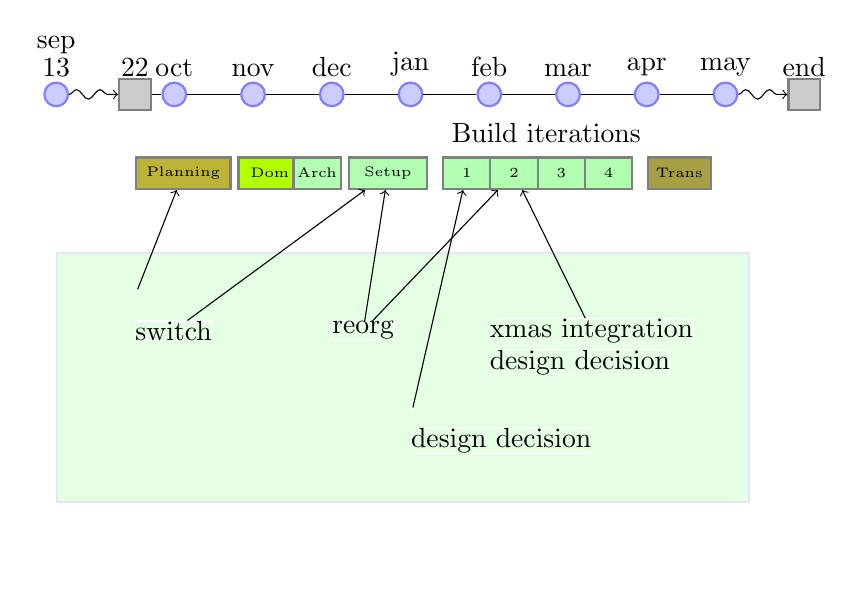
\begin{tikzpicture}
 	[month/.style={circle,draw=blue!50,fill=blue!20,thick,inner sep=0pt,minimum size=3mm},
	transition/.style={rectangle,draw=black!50,fill=black!20,thick,inner sep=0pt,minimum size=4mm},
	iteration/.style={rectangle,draw=black!50,fill=green!30,anchor=west,thick,
				inner sep=0pt,minimum height=4mm, minimum width=6mm},
	orgiter/.style={rectangle,draw=black!50,fill=yellow!60!black,anchor=west,thick,
				inner sep=0pt,minimum height=4mm, minimum width=8mm},
	planiter/.style={rectangle,draw=black!50,fill=yellow!70!black,anchor=west,thick,
				inner sep=0pt,minimum height=4mm, minimum width=12mm},
	domainiter/.style={rectangle,draw=black!50,fill=green!30!yellow,anchor=west,thick,
				inner sep=0pt,minimum height=4mm, minimum width=8mm},
	setupiter/.style={rectangle,draw=black!50,fill=green!30,anchor=west,thick,
				inner sep=0pt,minimum height=4mm, minimum width=10mm},
	txt/.style={rectangle,draw=white,anchor=west,thin, inner sep=0pt},
	events/.style={rectangle,draw=blue!10,fill=green!10,inner sep=0pt,thick,minimum height=9em, minimum width=25em,anchor=north west}
				]
%%	[fill=green!70!blue,every path/.style={draw}]
	\newcounter{ysize};
	\setcounter{ysize}{7};
	\newcommand{\y}{\value{ysize}}
	\node (sep) at (-0.5,\y-1)    [month] {};
	\node (start) at (0.5,\y-1) [transition] {};
	\node (oct) at (1.0,\y-1)  [month] {};
	\node (nov) at (2.0,\y-1)    [month] {};
	\node (dec) at (3.0,\y-1)  [month] {};
	\node (jan) at (4.0,\y-1)    [month] {};
	\node (feb) at (5.0,\y-1)  [month] {};
	\node (mar) at (6.0,\y-1)    [month] {};
	\node (apr) at (7.0,\y-1) [month] {};
	\node (may) at (8.0,\y-1)   [month] {};
	\node (end) at (9.0,\y-1)   [transition] {};
	\path (0,0);
	\node (planning) at (0.5, \y-2) [planiter] {\tiny Planning};
	\node (domain) at (1.8, \y-2) [domainiter] {\tiny Dom};
	\node (arch) at (2.5, \y-2) [iteration] {\tiny Arch};
	\node (setup) at (3.2, \y-2) [setupiter] {\tiny Setup};
	\node (iterA) at (4.4, \y-2) [iteration] {\tiny 1};
	\node [above=3mm of iterA.north west,anchor=west] {Build iterations};
	\node (iterB) at (5.0, \y-2) [iteration] {\tiny 2};
	\node (iterC) at (5.6, \y-2) [iteration] {\tiny 3};
	\node (iterD) at (6.2, \y-2) [iteration] {\tiny 4};
	\node (transition) at (7.0,\y-2) [orgiter] {\tiny Trans}; 
	\draw (sep) node[above=11pt] {sep};
	\draw (sep) node[above=3pt] {13};
	\draw (start) node[above=3pt] {22};
	\draw (oct) node[above=3pt] {oct};
	\draw (nov) node[above=3pt] {nov};
	\draw (dec) node[above=3pt] {dec};
	\draw (jan) node[above=3pt] {jan};
	\draw (feb) node[above=3pt] {feb};
	\draw (mar) node[above=3pt] {mar};
	\draw (apr) node[above=3pt] {apr};
	\draw (may) node[above=3pt] {may};
	\draw (end) node[above=3pt] {end};
	\draw (start) -- (oct) -- (nov) -- (dec) -- (jan) -- (feb) -- (mar) -- (apr) -- (may);
	\draw [->,decorate,decoration={snake,amplitude=.6mm,segment length=3mm,post length=1mm}] (sep) -- (start);
	\draw [->,decorate,decoration={snake,amplitude=.6mm,segment length=3mm,post length=1mm}] (may) -- (end);

	\node (events) at (-0.5, \y-3) [events] {};
	\node (dad) at (0.5, \y-3.5) [txt] {\dad};
	\draw [->,decorate] (dad) -- (planning);
	\node (qtswitch) at (0.5, \y-4) [txt] {\qt switch};
	\draw [->,decorate] (qtswitch) -- (setup);
	\node (qtqml) at (4.0, \y-5) [txt] {\qt \qml};
	\node (qtqmlD) at (4.0, \y-5.4) [txt] {design decision};
	\draw [->,decorate] (qtqml) -- (iterA);
	\node (oureorg) at (3.0, \y-4) [txt] {\ou reorg};
	\draw [->,decorate] (oureorg) -- (setup);
	\draw [->,decorate] (oureorg) -- (iterB);
	\node (xintegr)  at (5.0, \y-4) [txt] {xmas integration};
	\node (xintegrD) at (5.0, \y-4.4) [txt] {design decision};
	\draw [->,decorate] (xintegr) -- (iterB);
	

%    % draw vertical lines
%    \foreach \x in {0,1,2,4,5,7}
%      \draw (\x cm,3pt) -- (\x cm,-3pt);

  \end{tikzpicture}
\end{frame}


\begin{frame}[t]{Product \& technology}
	\begin{itemize}
		\item \textbf{Agilefant}
		\item \textbf{Qt Quick2}
		\item \textbf{product demo}
		\item \textbf{contribution}
	\end{itemize}	
	
\end{frame}
  
\begin{frame}{Agilefant tool}
	\begin{columns}
		\begin{column}[t]{5cm}
			\textbf{DAD:}
			\begin{itemize}
				\item visualize work
				\item backlog
				\item automated metrics
			\end{itemize}
		\end{column}
		\pause
		\begin{column}[t]{5cm}
			\textbf{Agilefant:}		
			\begin{itemize}
				\item open source
				\item web hosted tool
				\item backlog \& metrics
				\item stories, iterations, tasks
				\item visualize \& prioritize work		
			\end{itemize}		
		\end{column}
	\end{columns}
	\begin{center}
		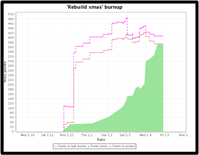
\includegraphics[width=.30\linewidth]{pictures/af-metrics}
		\hspace{0.5cm}	
		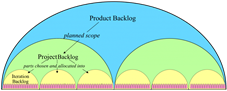
\includegraphics[width=.50\linewidth]{pictures/af-elephant}
	\end{center}
		
\end{frame}

\begin{frame}{Agilefant backlog}
	\begin{center}
		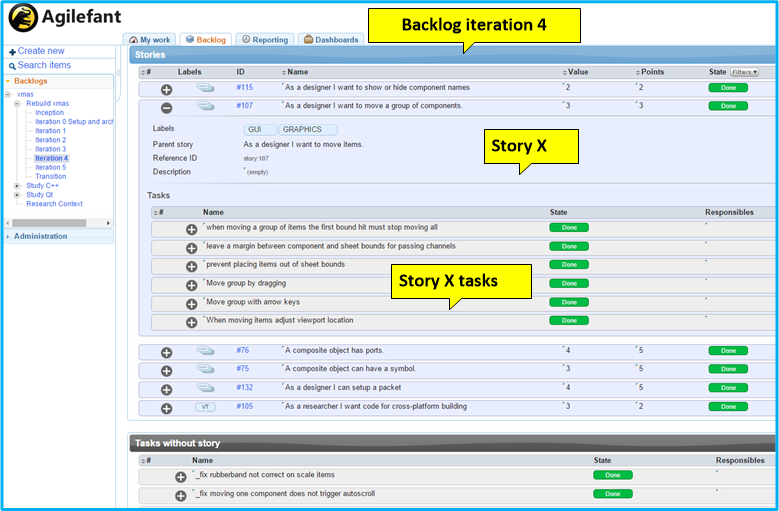
\includegraphics[width=0.9\linewidth]{pictures/backlog}
	\end{center}
\end{frame}

\begin{frame}{Qt Quick2}
	\begin{columns}
		\begin{column}[t]{5cm}
			{\bf FLTK?}
			\begin{itemize}
				\item graphics library only
				\item basic widgets.
				\item pure c++
				\item no native look-and-feel
				\item create from scratch
			\end{itemize}
			\pause
			{\bf Qt Quick1?}
			\begin{itemize}
				\item not for future designs
				\item painter raster rendering
				\item native desktop widgets
			\end{itemize}
		\end{column}
		\pause
		\begin{column}[t]{5cm}
			\textbf{Qt Quick2!}
			\begin{itemize}
				\item all-in-one environment
				\item declarative UI language QML (JavaScript+)
				\item separate back-end (c++) enforces model/view
				\item signals \& slots
				\item OpenGL 2.0
			\end{itemize}
		\end{column}
	\end{columns}
\end{frame}

\begin{frame}[t]{Qt Quick2}
	\textbf{Registered c++ class $\rightarrow$ instantiable QML type}
	\begin{center}
		\only<1>{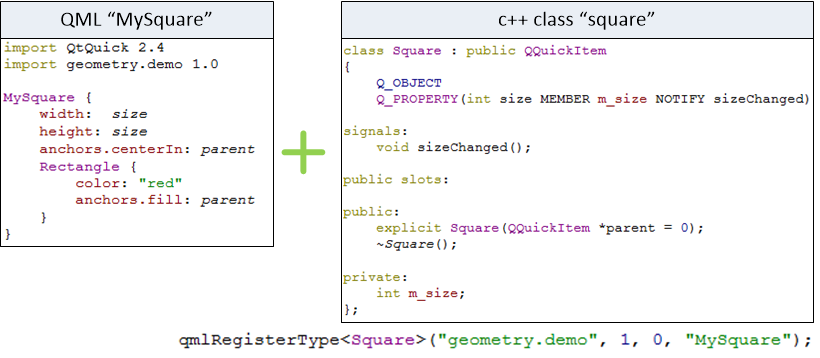
\includegraphics[width=.90\linewidth]{pictures/qml1}}
		\only<2>{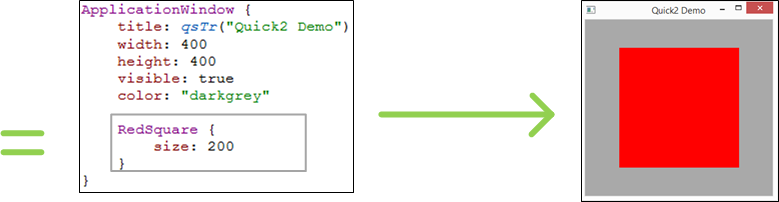
\includegraphics[width=.90\linewidth]{pictures/qml2}}
	\end{center}
\end{frame}

\begin{frame}[t]{Qt Quick2}
	\textbf{Embedded c++ class  $\rightarrow$ QML context}
	\begin{center}
		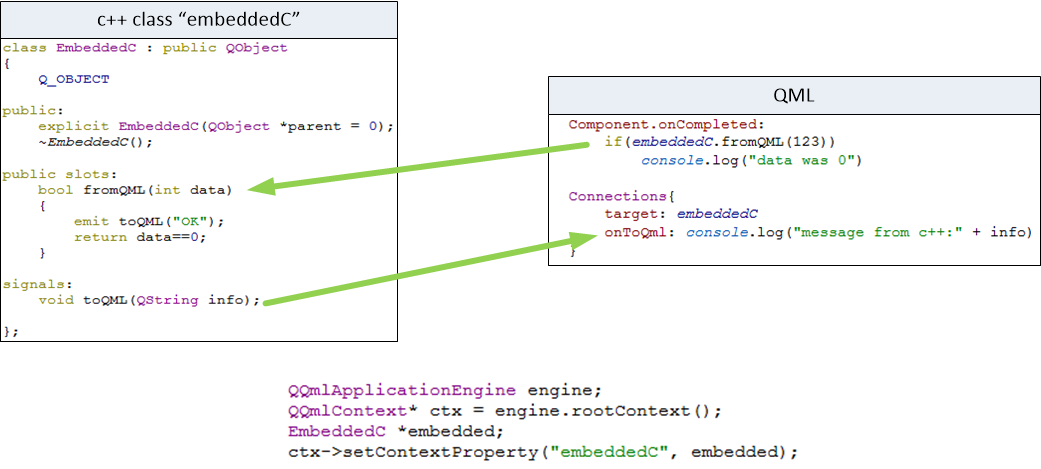
\includegraphics[width=.90\linewidth]{pictures/qml3}
	\end{center}
\end{frame}


%% Demo XMAS Designer
\begin{frame}{Demo ``xmd'' \underline{x}MAS \underline{m}odel \underline{d}esigner}

	\begin{columns}
		\begin{column}[b]{0.8\textwidth}
			\begin{itemize}
				\item built with Qt Quick2 technology
				\item easy and powerful QML JavaScript GUI language
				\item c++ logic interfacing
				\item signal-slot event handling
				\item platform independent
			\end{itemize}			
		\end{column}
		\begin{column}[c]{.5\textwidth}
			
\includegraphics[width=0.75\linewidth]{pictures/2a-xmd}
		\end{column}
	\end{columns}
		
\end{frame}

\begin{frame}{xmd - main application window}
	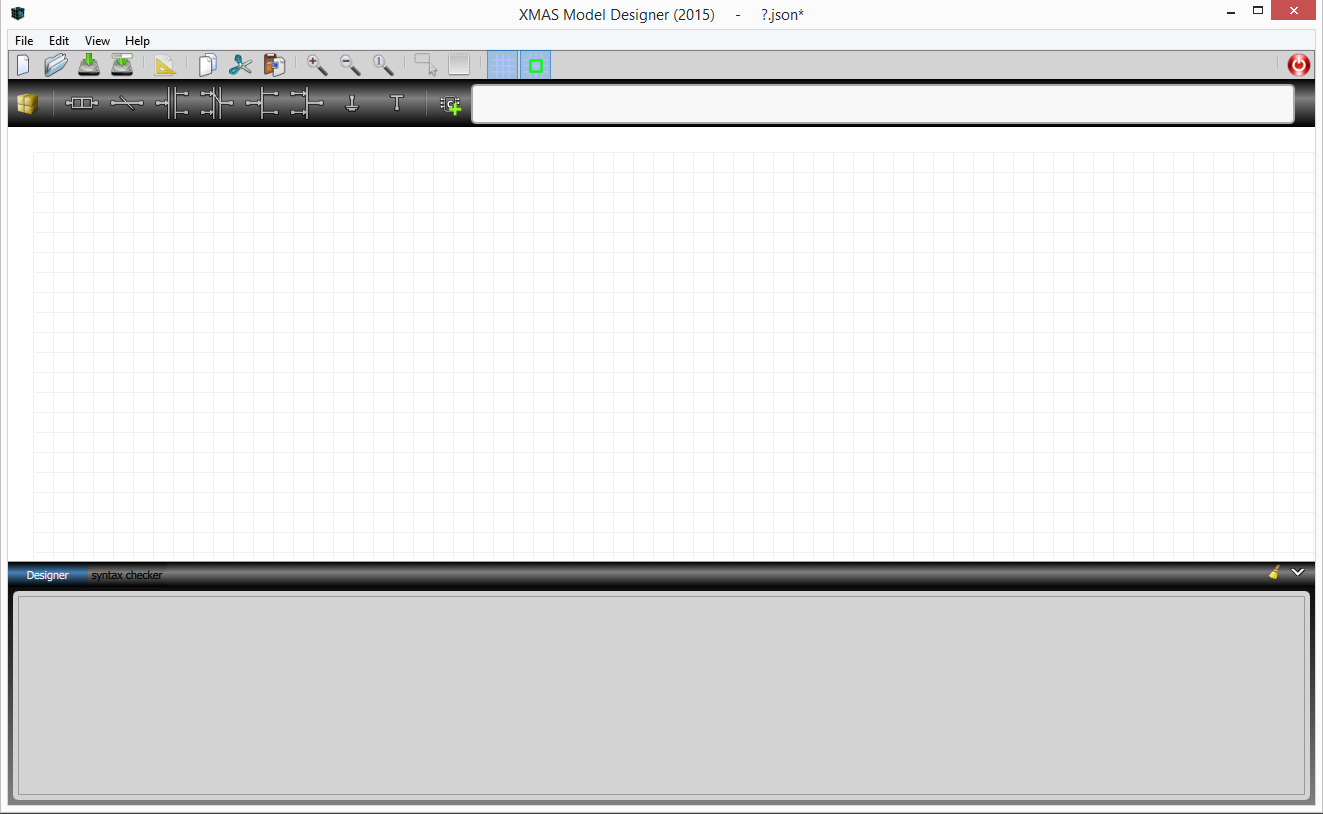
\includegraphics[width=.90\linewidth]{pictures/2b-xmd-empty}
\end{frame}
\begin{frame}{xmd - application setup}
	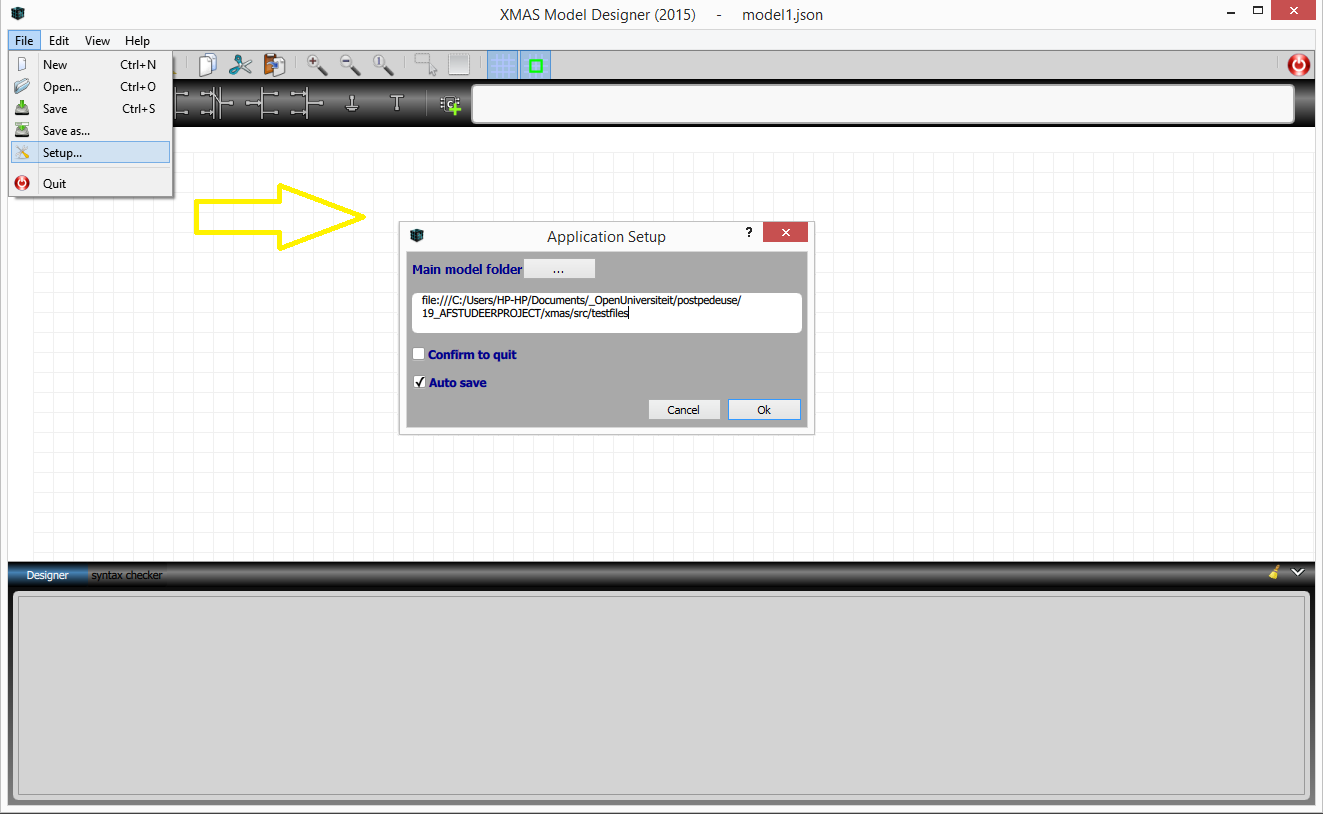
\includegraphics[width=.90\linewidth]{pictures/2c-xmd-app-setup}
\end{frame}
\begin{frame}{xmd - model setup}
	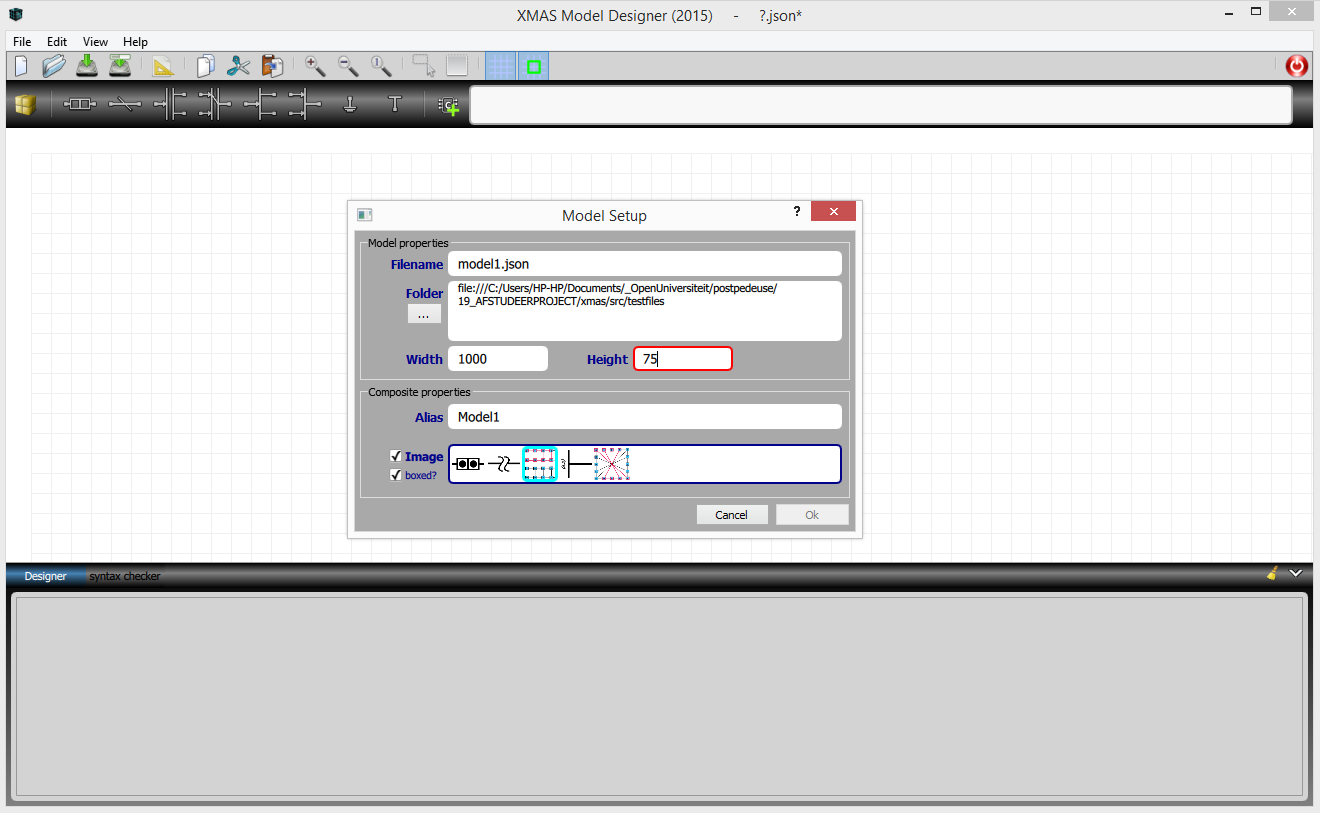
\includegraphics[width=.90\linewidth]{pictures/2d-xmd-model-setup}
\end{frame}
\begin{frame}{xmd - canvas}
	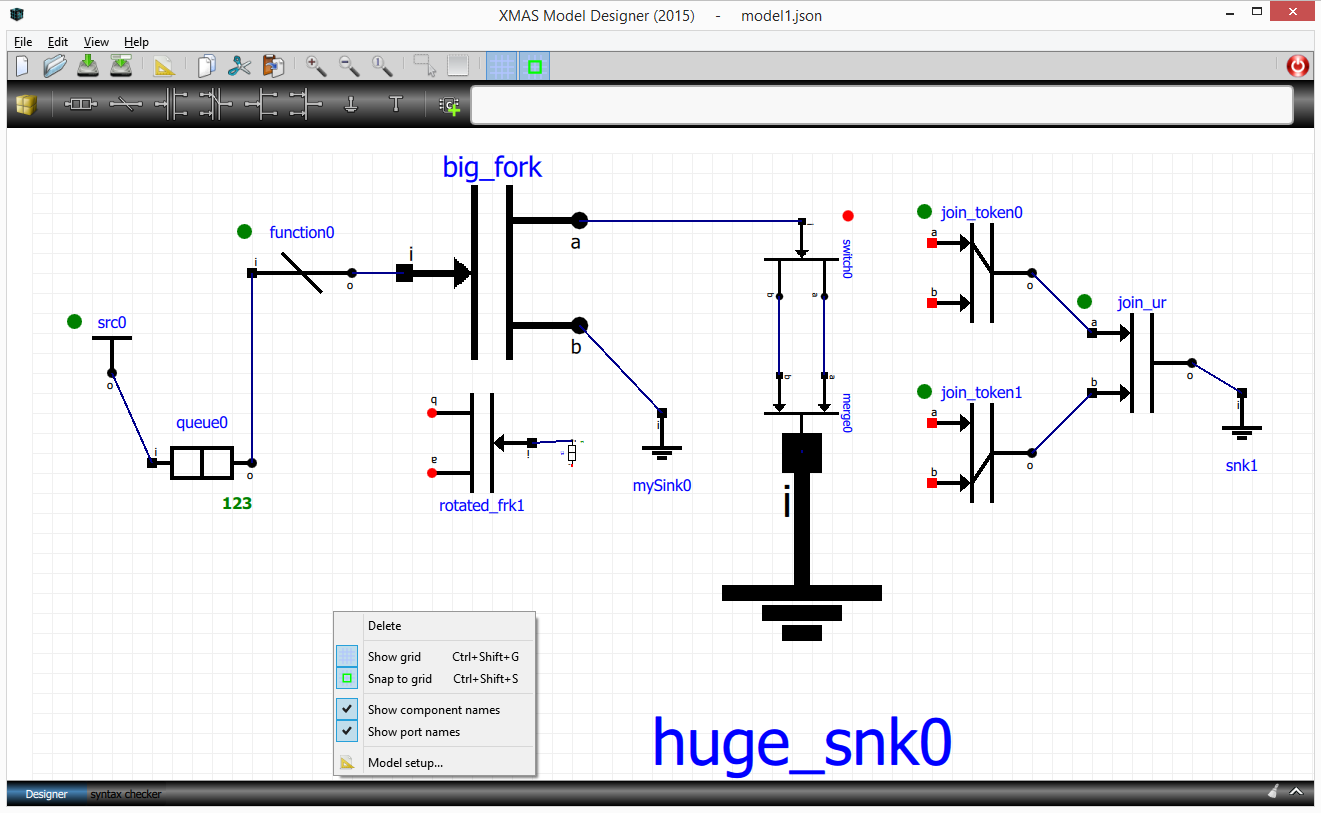
\includegraphics[width=.90\linewidth]{pictures/2e-xmd-canvas}
\end{frame}
\begin{frame}{xmd - group select}
	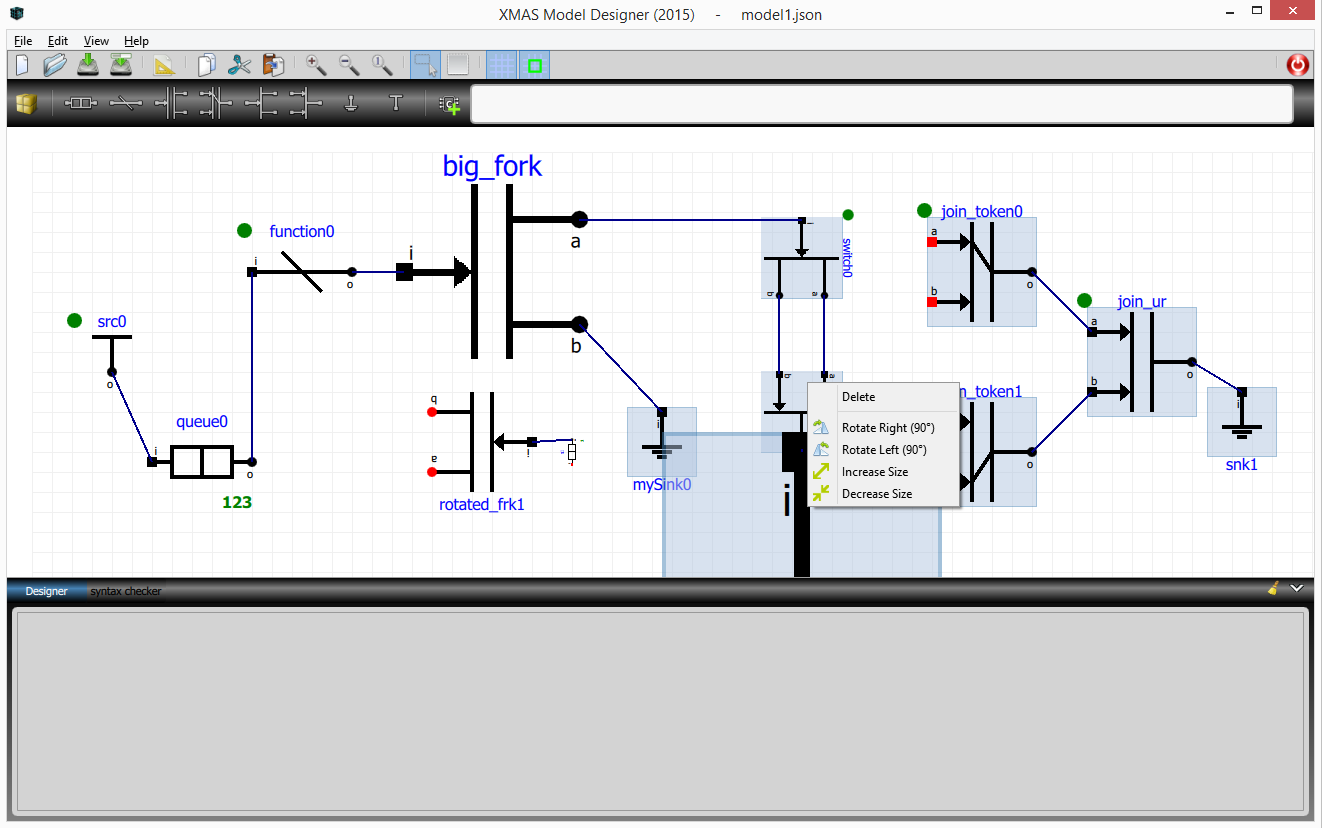
\includegraphics[width=.90\linewidth]{pictures/2f-xmd-canvas-groupselect}
\end{frame}
\begin{frame}{xmd - group delete}
	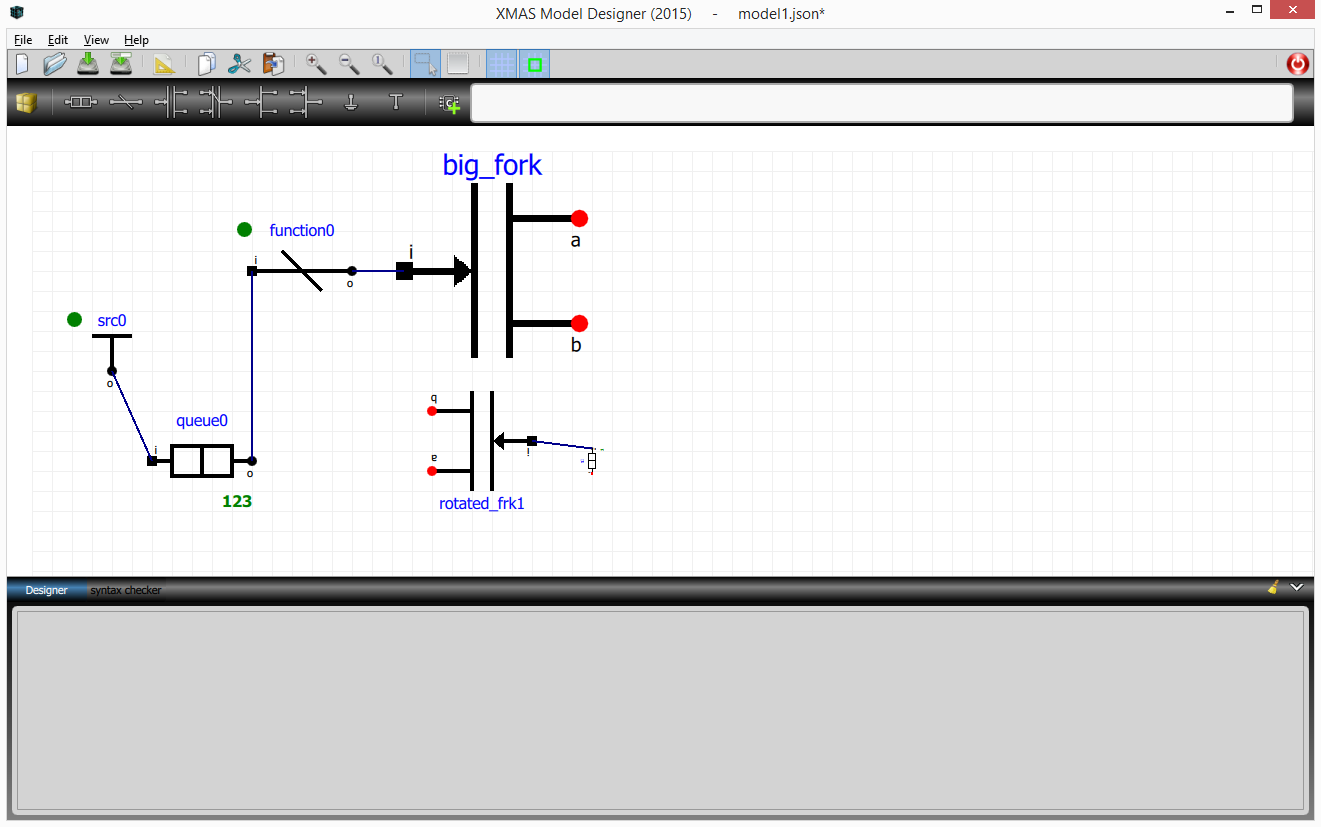
\includegraphics[width=.90\linewidth]{pictures/2g-xmd-canvas-delete}
\end{frame}
\begin{frame}{xmd - expression error feedback}
	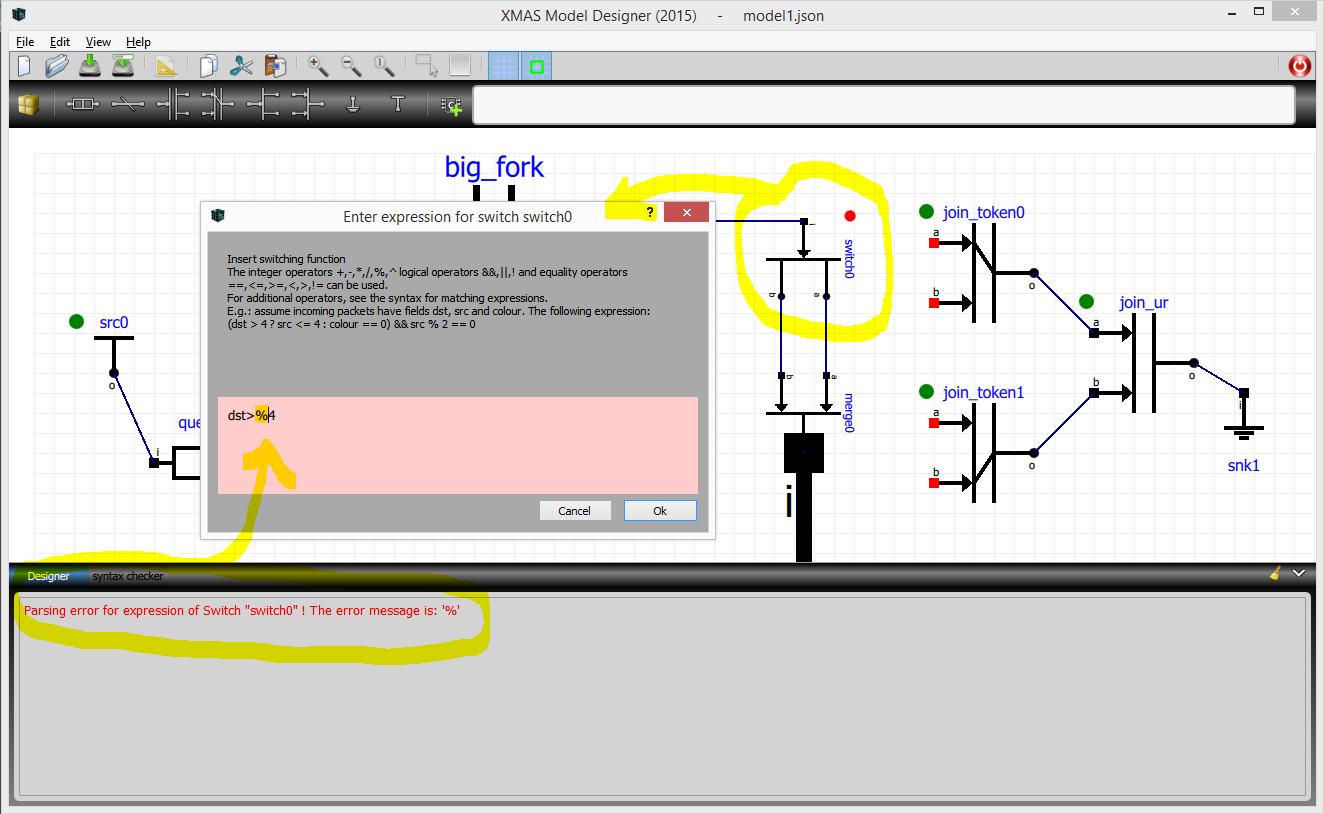
\includegraphics[width=.90\linewidth]{pictures/2h-xmd-expressiondialog-error}
\end{frame}
\begin{frame}{xmd - expression valid feedback}
	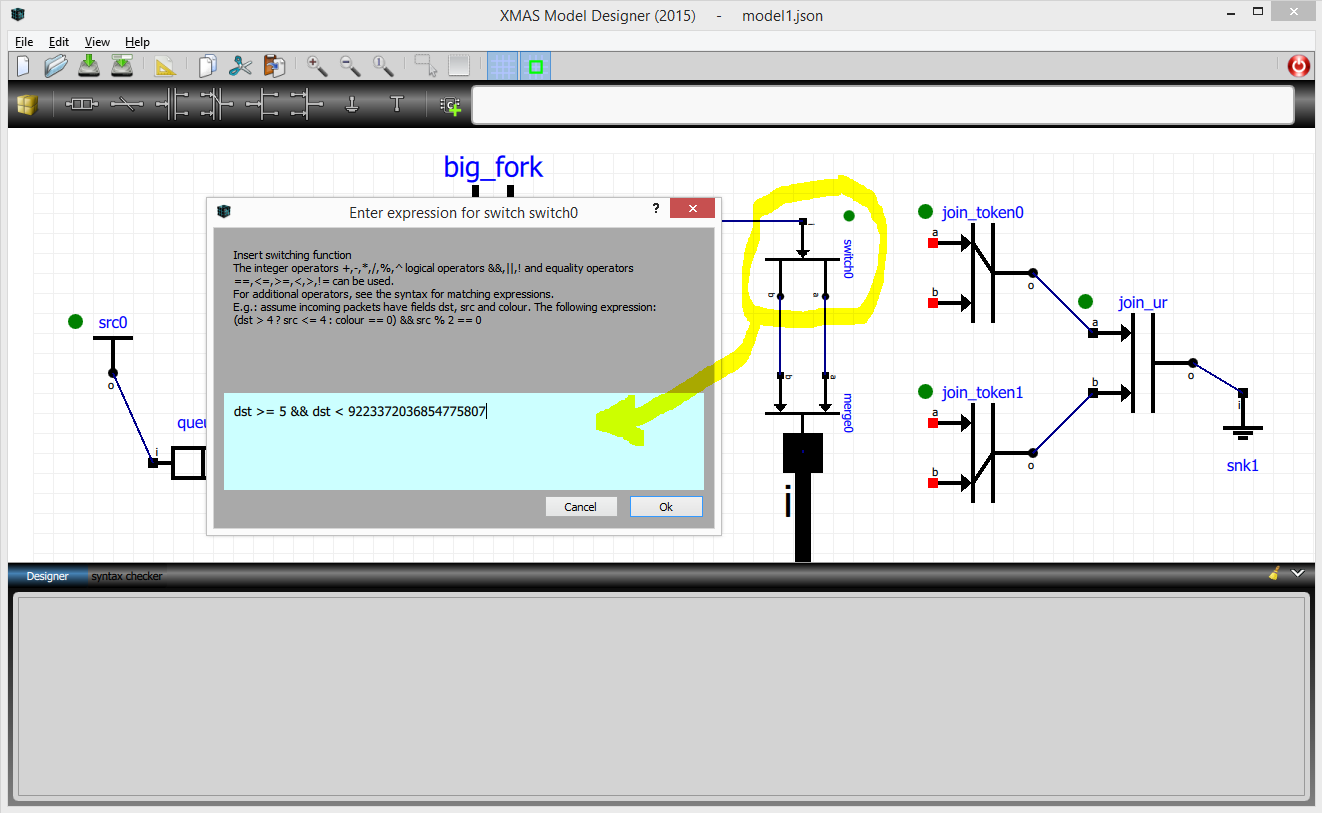
\includegraphics[width=.90\linewidth]{pictures/2i-xmd-expressiondialog-valid}
\end{frame}
\begin{frame}{xmd - composite library ``add''}
	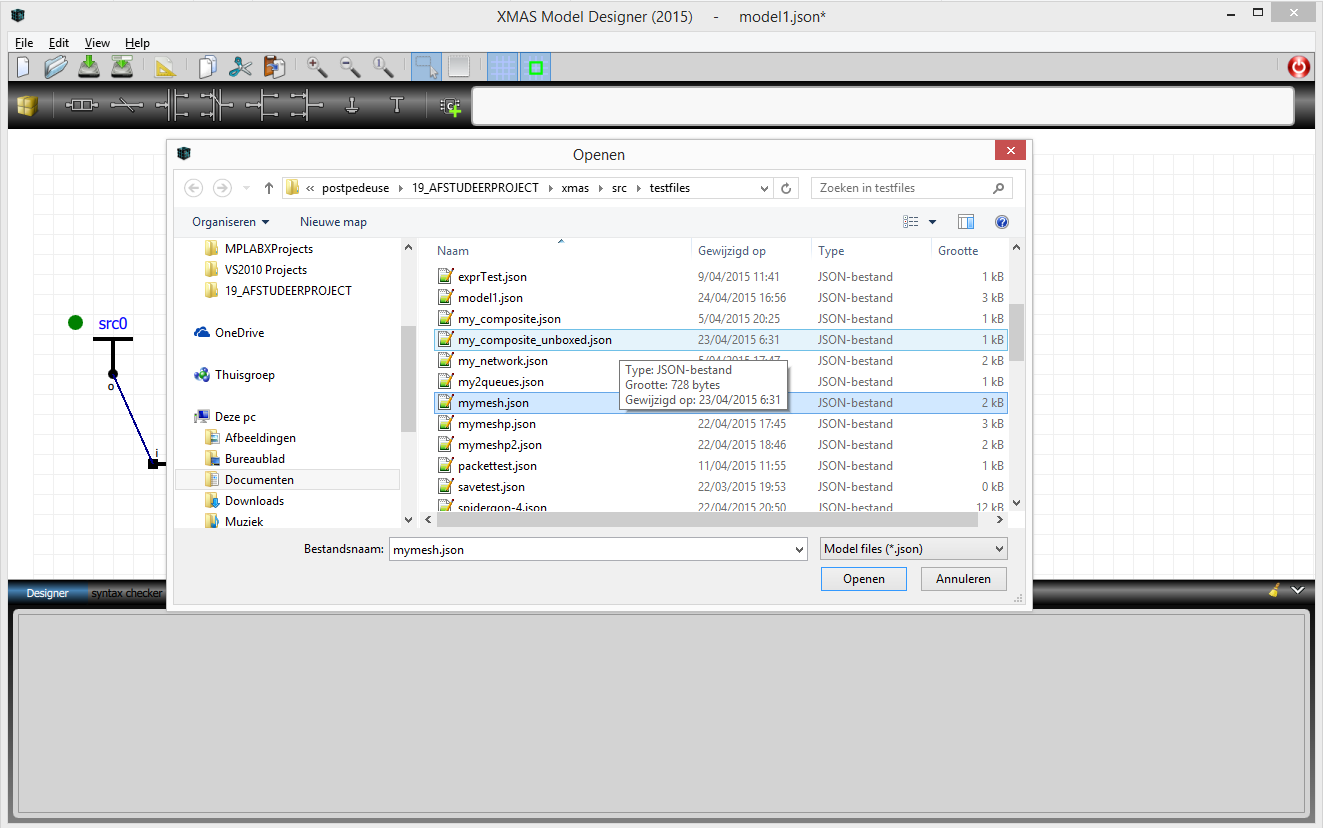
\includegraphics[width=.90\linewidth]{pictures/2j-xmd-compositelibrary-add}
\end{frame}
\begin{frame}{xmd - composite library ``remove''}
	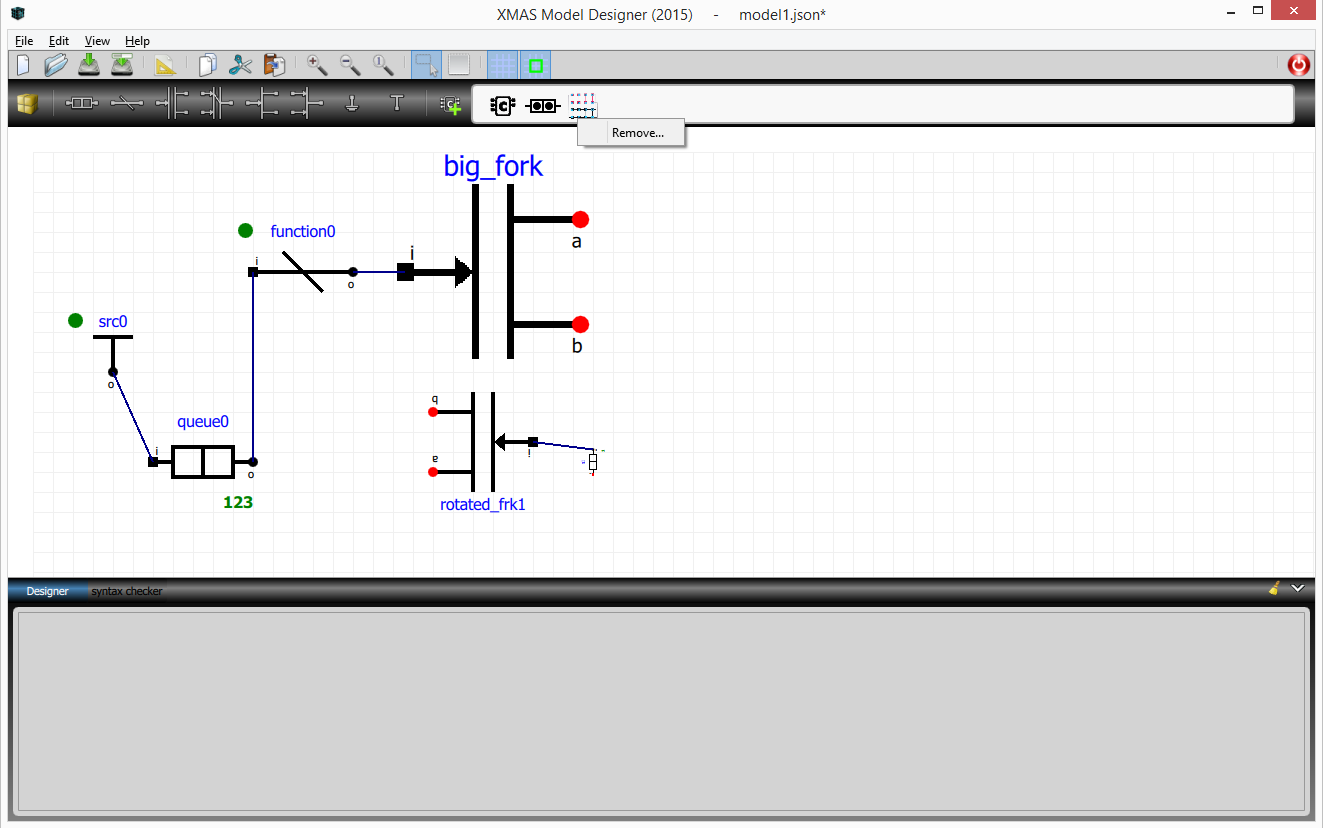
\includegraphics[width=.90\linewidth]{pictures/2k-xmd-compositelibrary-remove}
\end{frame}
\begin{frame}{xmd - composite use}
	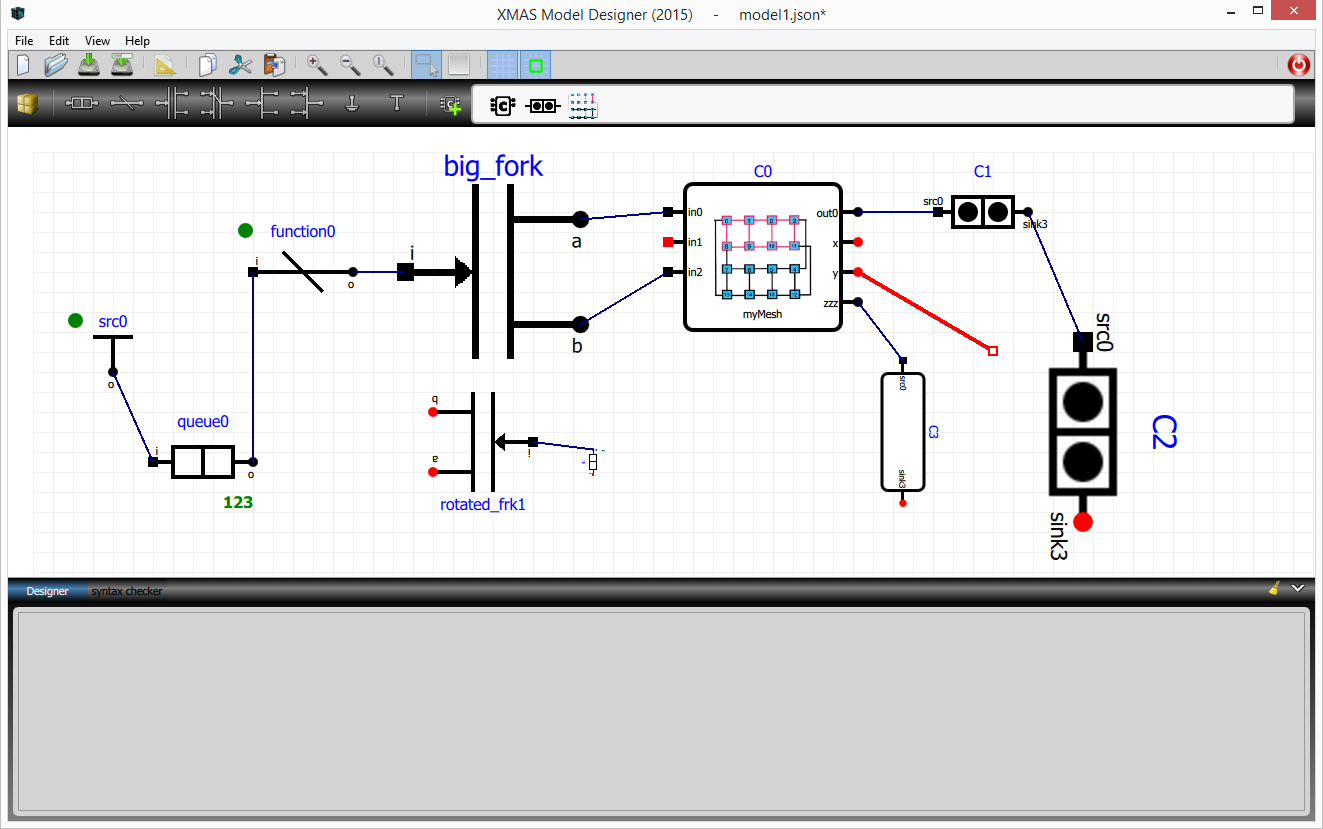
\includegraphics[width=.90\linewidth]{pictures/2l-xmd-composite-use}
\end{frame}
\begin{frame}{xmd - plug in}
	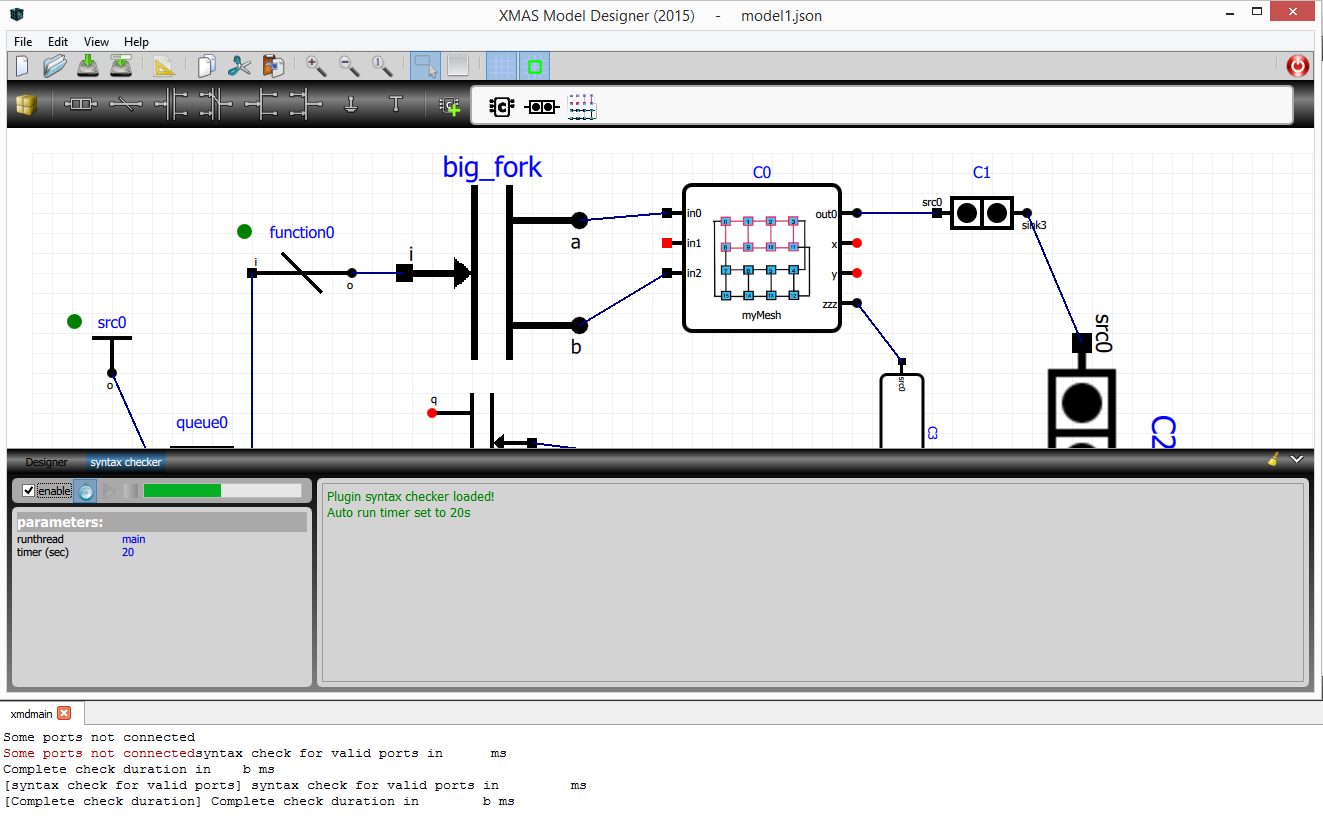
\includegraphics[width=.90\linewidth]{pictures/2m-xmd-plug-in}
\end{frame}
%% Demo XMAS Designer (end)

%% what are the benefits
\begin{frame}[t]{Contribution to research project}

	\begin{itemize}
		\item Integration of formal verification   $\rightarrow$  Designer friendly \\
		= get benefits without complexity concerns.
		\item Multi-platform $\rightarrow$ More researchers can make use if this tool \\
		= more interest.
		\item Maintainability   $\rightarrow$ The better to maintain the easier to adjust \\
		= satisfied users.
		\item Technology   $\rightarrow$ Qt well known IDE \\
		= support.		
	\end{itemize}
\end{frame}



\begin{frame}{Specification model Data Layer iteration 1}

	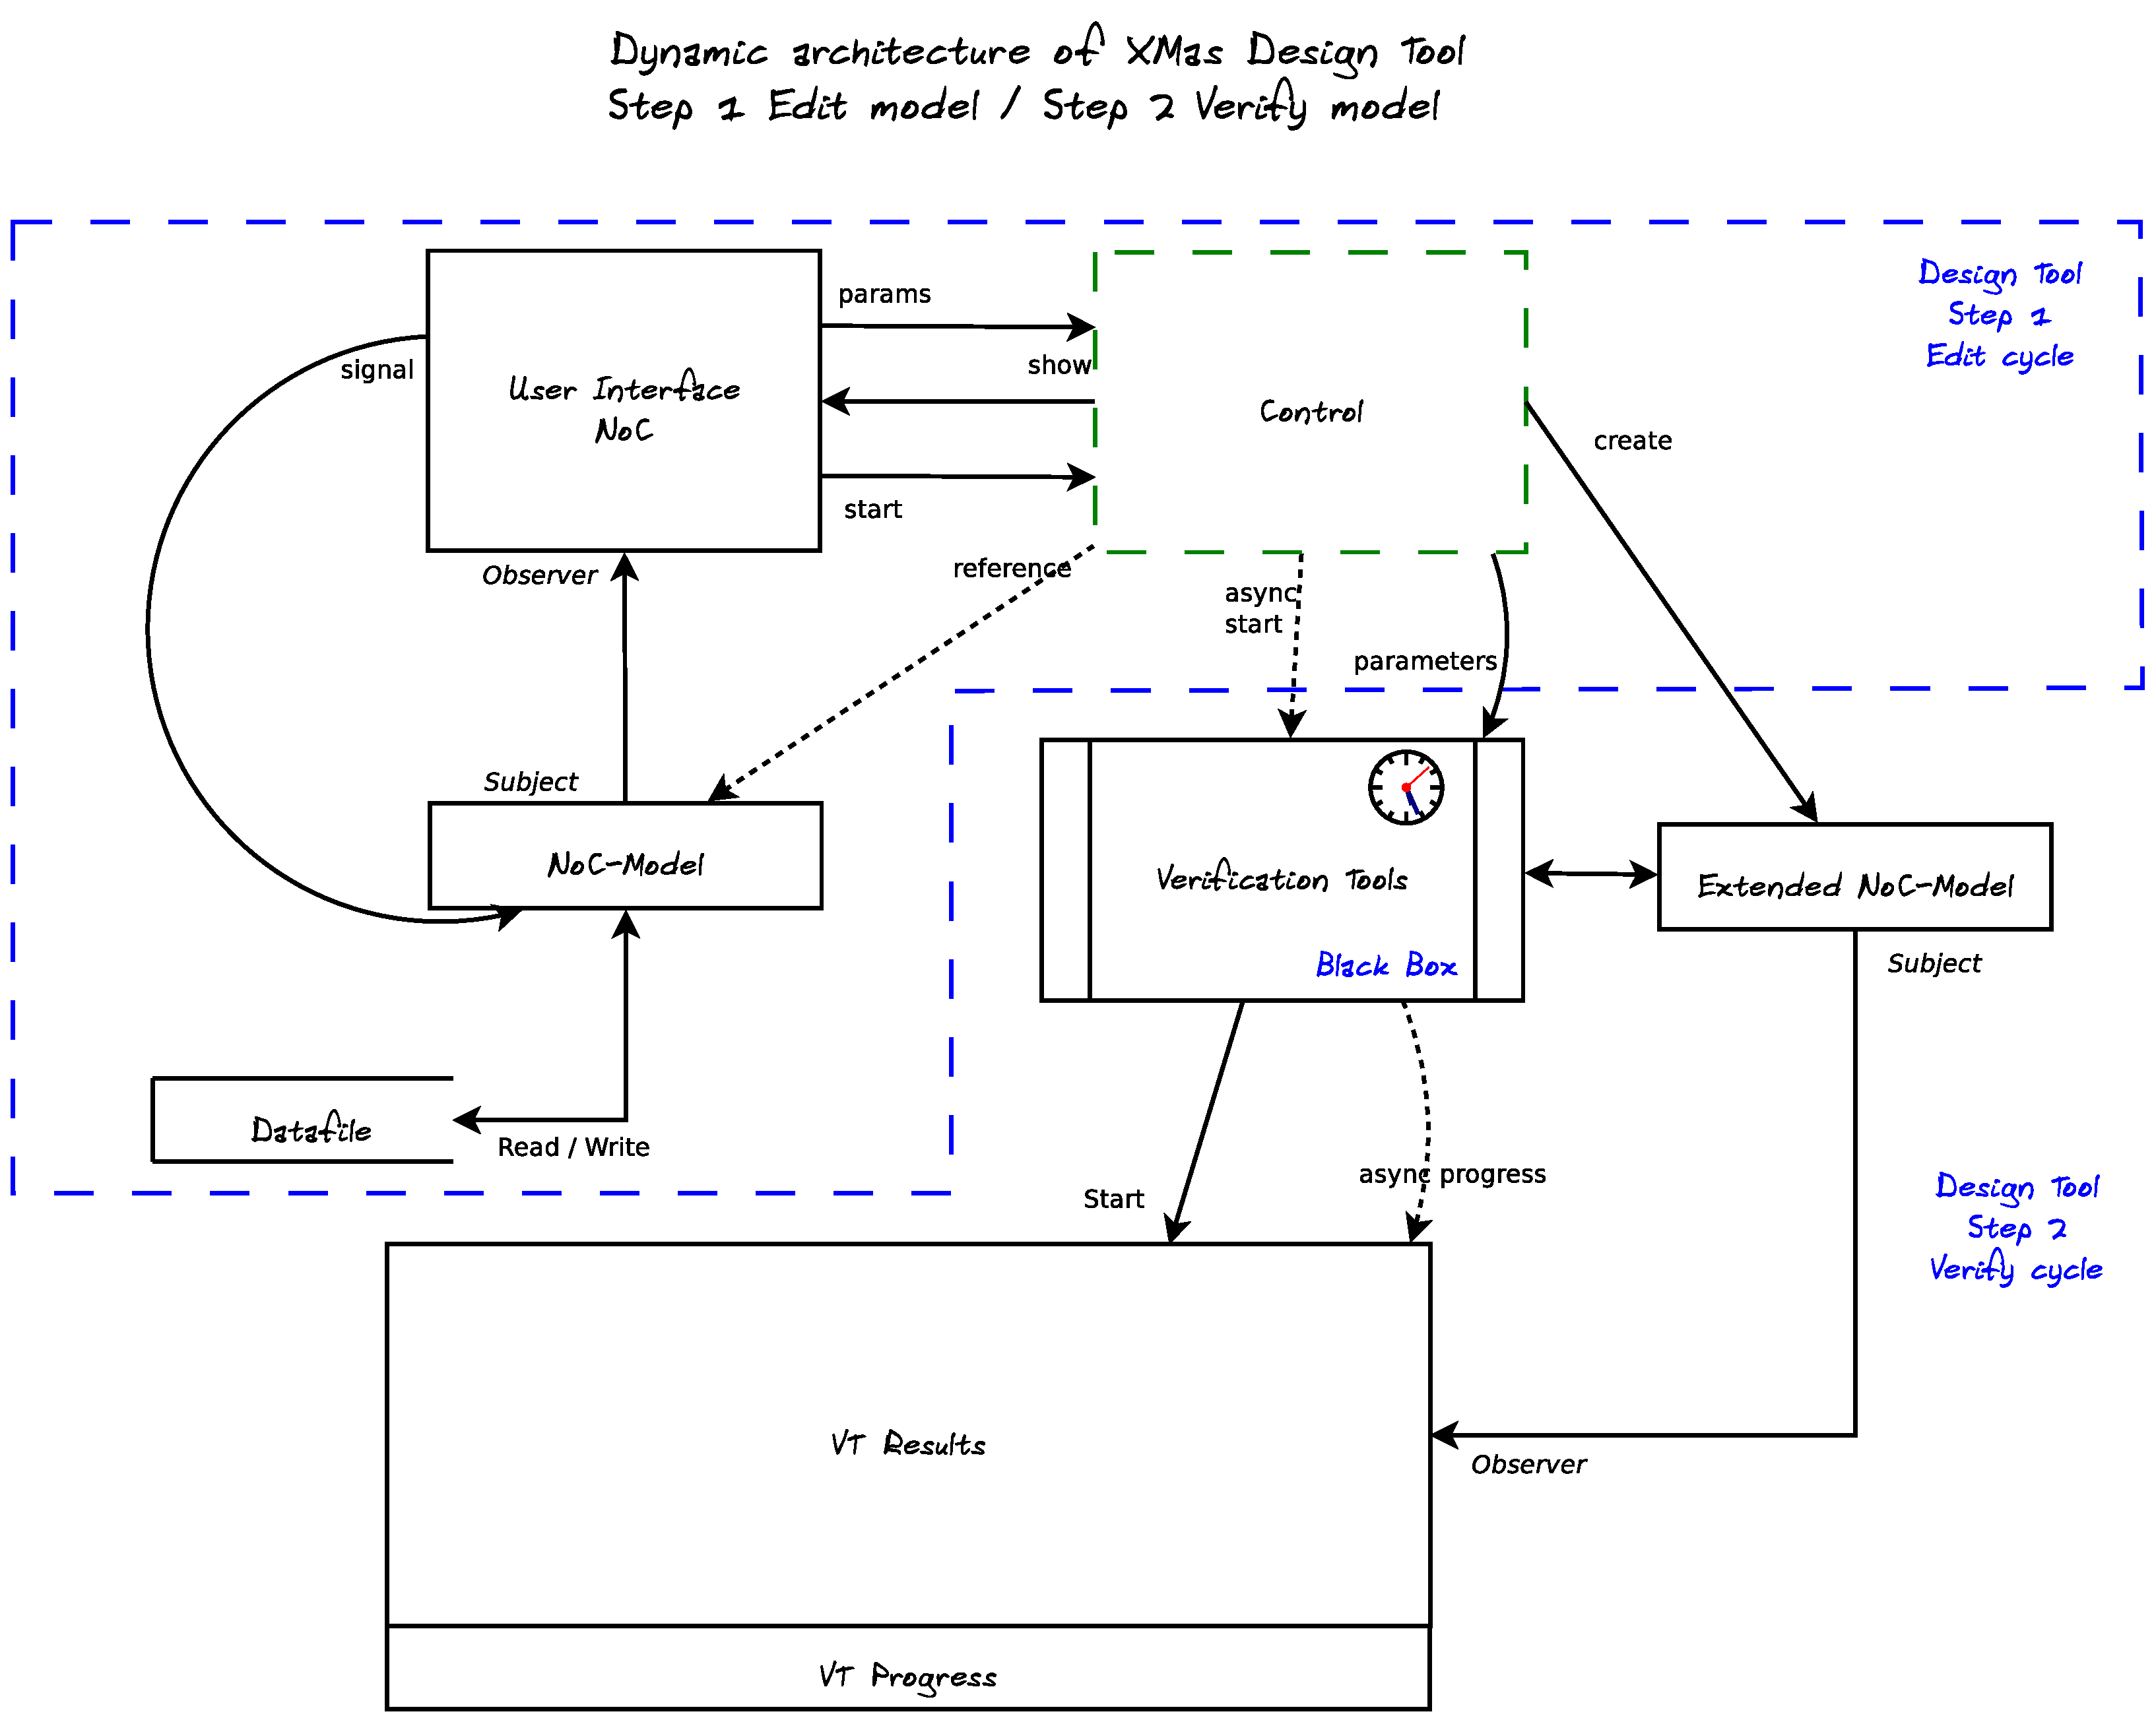
\includegraphics[width=.80\linewidth]{pictures/1c-architecture-dynamic-1}

\end{frame}

\begin{frame}{Implementation Data layer}

	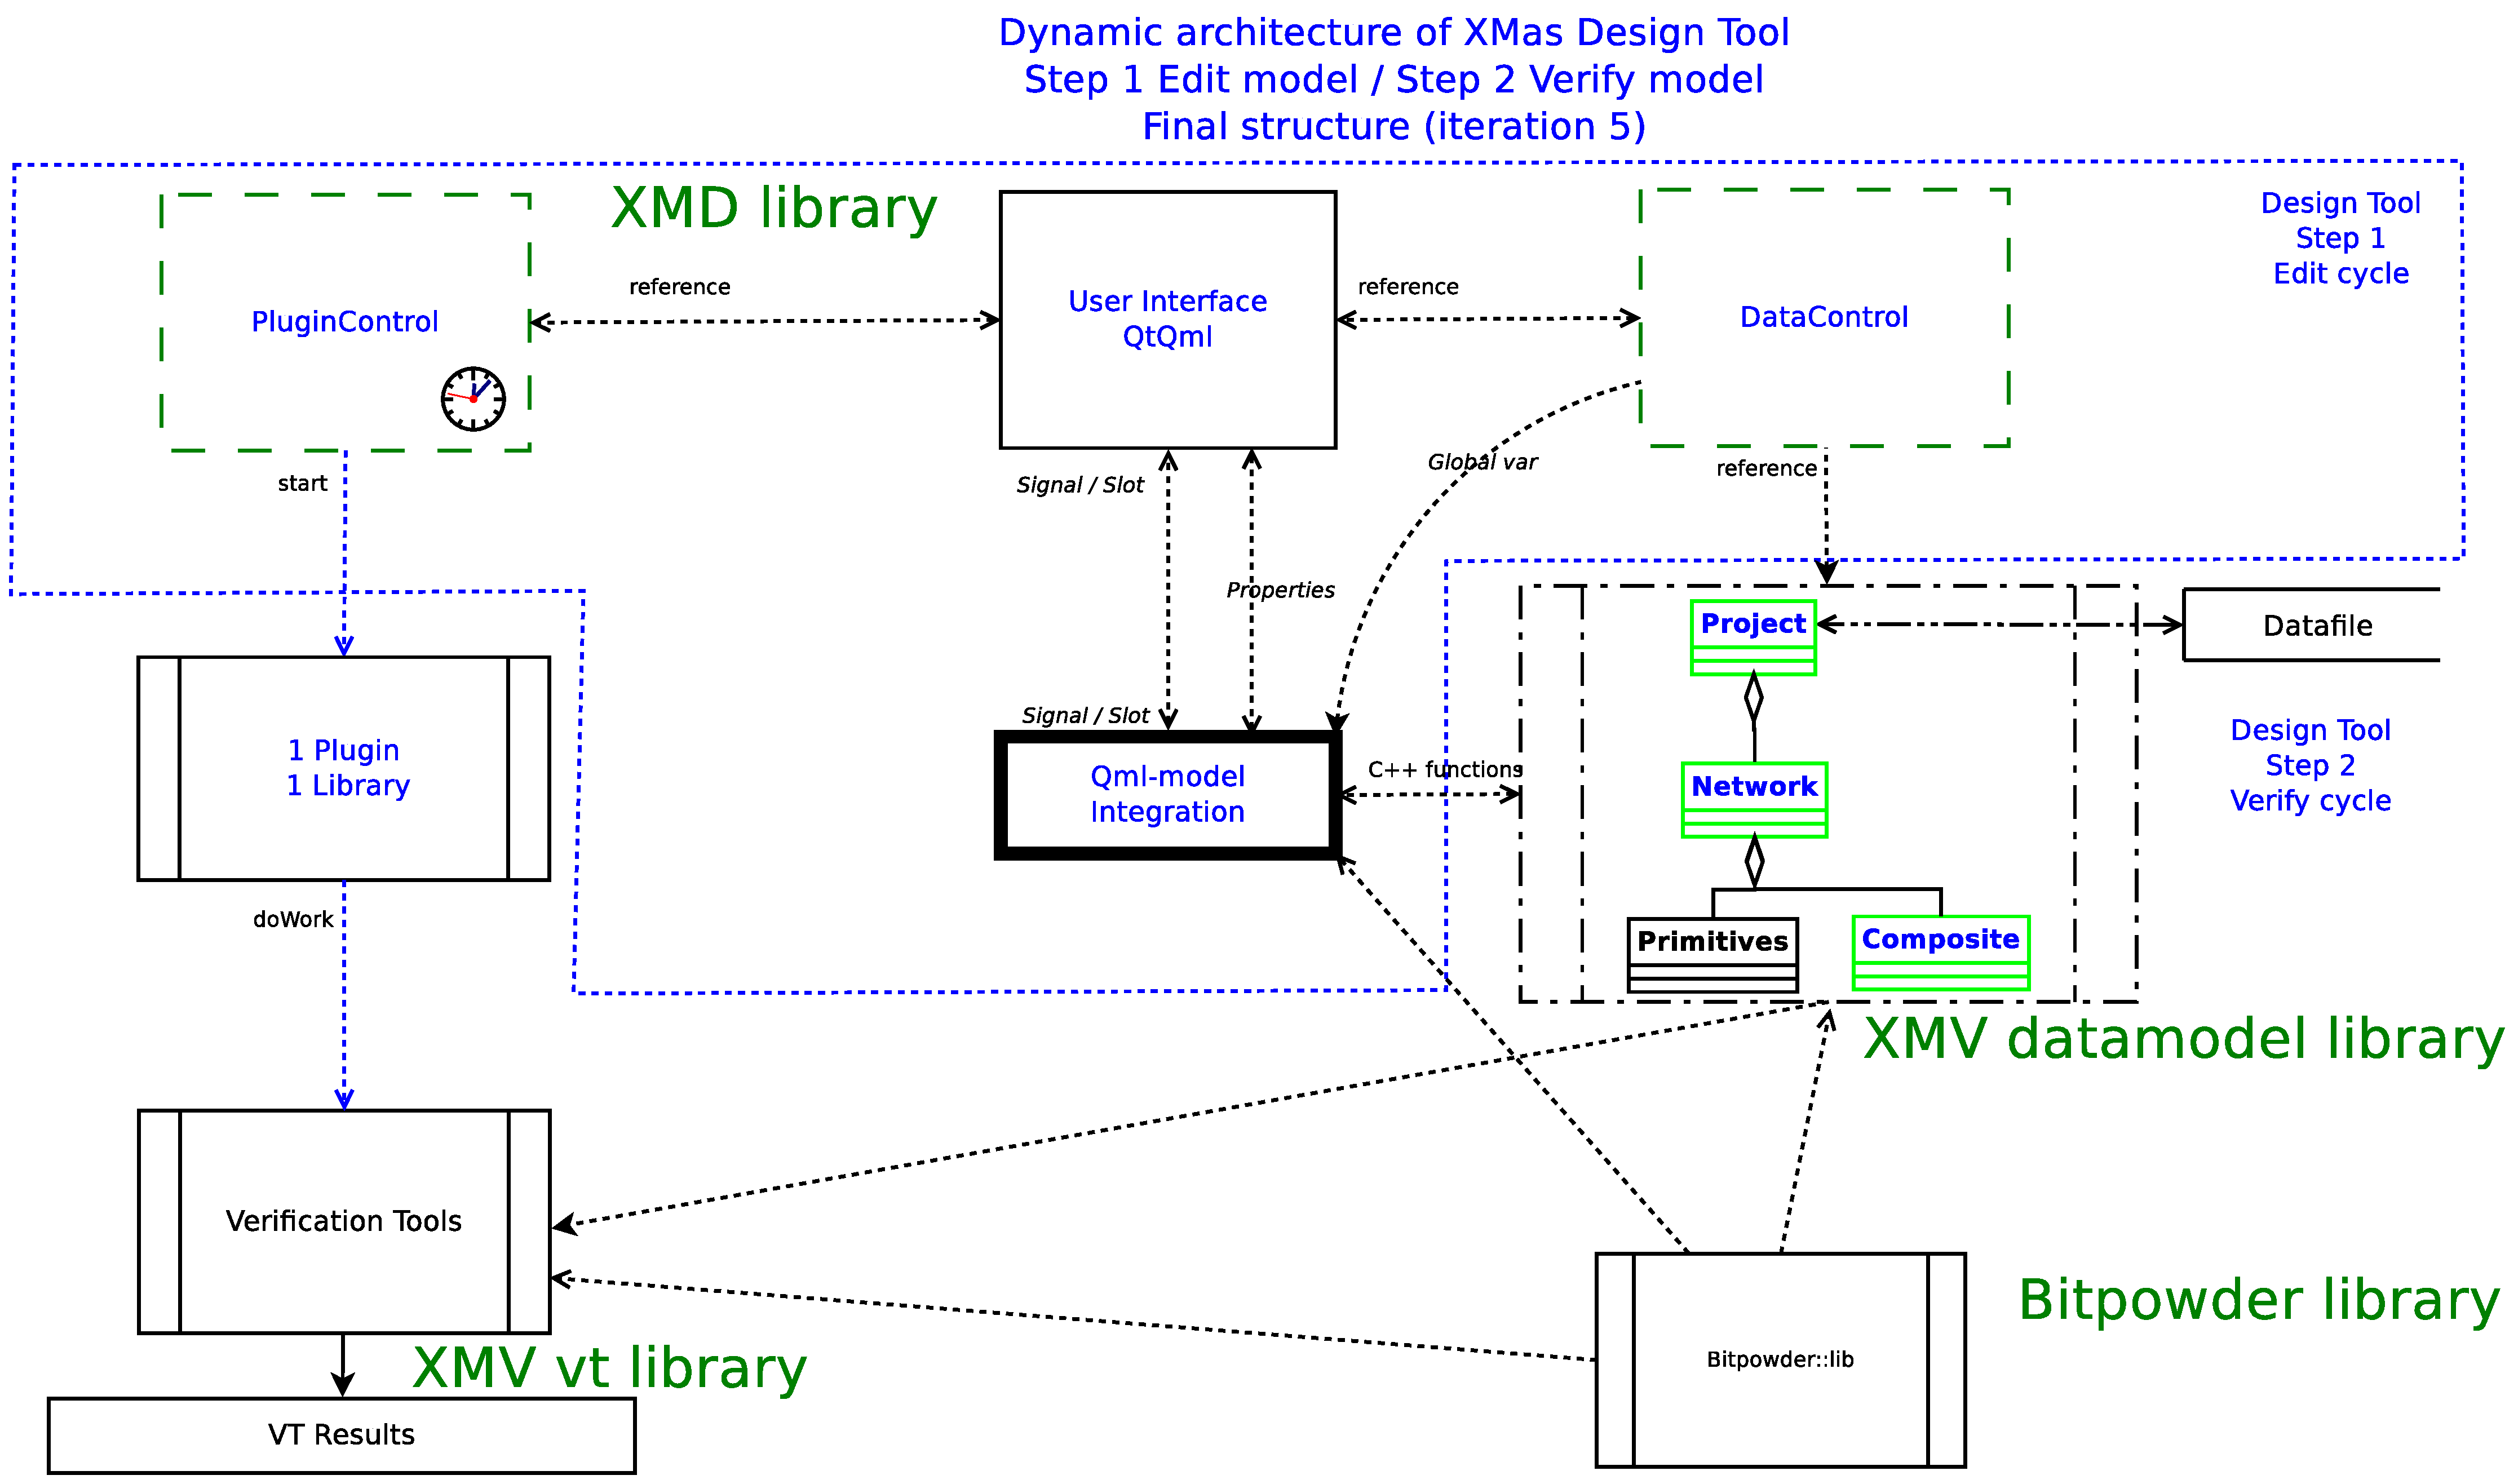
\includegraphics[width=.90\linewidth]{pictures/1c-architecture-dynamic-2}

\end{frame}

\begin{frame}{Process Reflection}
	\begin{itemize}
		\item {\bf Agile} 
				\begin{itemize}
					\item tools: skype: teamviewer, github, agilefant. Worked well.
					\item Internal communication: worked very well
					\item External communication: limited due to OU reorganisation
				\end{itemize}
		\item {\bf Planning}
				\begin{itemize}
					\item scheduling \& iterations: followed to a t.
					\item Influence OU reorg: risks increased
				\end{itemize}
		\item {\bf Design} 
			\begin{itemize}
				\item Switching to \qt				 (would do it again)
				\item Switching to \qml				 (would do it again)
				\item Switching to tight xmas integration (underestimated consequences)
			\end{itemize}
	\end{itemize}
\end{frame}

\begin{frame}{Product Reflection}
	\begin{itemize}
		\item {\bf User Interface} 
				\begin{itemize}
					\item Programming user interface in \qml worked out well.
							It was a lot easier than the conventional user interface
					\item Integration between user interface and data structures
							was painfull. For next time take more serious note
							of alternatives affecting coupling through an interface
					\item Composites finished ok. Was easier due to \qml
				\end{itemize}
		\item {\bf Data structures}
				\begin{itemize}
					\item Extensions (useful for visiting pattern) were a source
							of memory errors, that partly still existed when
							released. They are still being worked on.
					\item Composites: easy enough to create. It shows the way
							for parameterized objects.
					\item Getting parsing right was more difficult than we expected.
				\end{itemize}
	\end{itemize}
\end{frame}

\begin{frame}
	\begin{description}
		\item[Source code] github https://github.com/bvgastel (Nog te bepalen)
		\item[Documentation] github repo
	\end{description}
\end{frame}

\end{document}
